% Options for packages loaded elsewhere
\PassOptionsToPackage{unicode}{hyperref}
\PassOptionsToPackage{hyphens}{url}
%
\documentclass[
  10pt,
  letterpaper,
]{article}
\usepackage{amsmath,amssymb}
\usepackage[margin=0.82in]{geometry}
\usepackage{amsthm}
\newtheorem{proposition}{Proposition}
\newtheorem{theorem}{Theorem}
\usepackage{iftex}
\ifPDFTeX
  \usepackage[T1]{fontenc}
  \usepackage[utf8]{inputenc}
  \usepackage{textcomp} % provide euro and other symbols
\else % if luatex or xetex
  \usepackage{unicode-math} % this also loads fontspec
  \defaultfontfeatures{Scale=MatchLowercase}
  \defaultfontfeatures[\rmfamily]{Ligatures=TeX,Scale=1}
\fi
\usepackage{lmodern}
\ifPDFTeX\else
  % xetex/luatex font selection
\fi
% Use upquote if available, for straight quotes in verbatim environments
\IfFileExists{upquote.sty}{\usepackage{upquote}}{}
\IfFileExists{microtype.sty}{% use microtype if available
  \usepackage[]{microtype}
  \UseMicrotypeSet[protrusion]{basicmath} % disable protrusion for tt fonts
}{}
\makeatletter
\@ifundefined{KOMAClassName}{% if non-KOMA class
  \IfFileExists{parskip.sty}{%
    \usepackage{parskip}
  }{% else
    \setlength{\parindent}{0pt}
    \setlength{\parskip}{6pt plus 2pt minus 1pt}}
}{% if KOMA class
  \KOMAoptions{parskip=half}}
\makeatother
\usepackage{xcolor}
\usepackage{graphicx}
\usepackage{flafter}
\usepackage{tikz}
\usetikzlibrary{arrows.meta,positioning}
\usepackage{longtable,booktabs,array}
\usepackage{calc} % for calculating minipage widths
% Correct order of tables after \paragraph or \subparagraph
\usepackage{etoolbox}
\makeatletter
\patchcmd\longtable{\par}{\if@noskipsec\mbox{}\fi\par}{}{}
\makeatother
% Allow footnotes in longtable head/foot
\IfFileExists{footnotehyper.sty}{\usepackage{footnotehyper}}{\usepackage{footnote}}
\makesavenoteenv{longtable}
\setlength{\emergencystretch}{3em} % prevent overfull lines
\providecommand{\tightlist}{%
  \setlength{\itemsep}{0pt}\setlength{\parskip}{0pt}}
\setcounter{secnumdepth}{5}
\ifLuaTeX
  \usepackage{selnolig}  % disable illegal ligatures
\fi
\IfFileExists{bookmark.sty}{\usepackage{bookmark}}{\usepackage{hyperref}}
\IfFileExists{xurl.sty}{\usepackage{xurl}}{} % add URL line breaks if available
\urlstyle{same}
\hypersetup{
  hidelinks,
  pdfcreator={LaTeX via pandoc}}

\title{Identification-Robust Inference for Complier\\
Cumulative-Incidence Effects under Competing Risks}
\author{Naresh Garg}
\date{19 August 2026}

\begin{document}
\maketitle

\begin{abstract}

Instrumental-variable analyses of competing-risk outcomes commonly
estimate a cause-specific complier cumulative-incidence effect by
dividing an intention-to-treat contrast in Aalen-Johansen cumulative
incidences by an intention-to-treat contrast in treatment uptake. This
ratio is regular only when compliance is bounded away from zero. We
propose a confidence set obtained by inverting the studentized,
undivided moment for a candidate complier effect. The procedure uses the
joint influence representation of the two Aalen-Johansen estimators and
the two treatment proportions, never divides by the estimated first
stage, and remains valid along triangular-array sequences in which the
compliance contrast is of order $n^{-1/2}$. The causal estimand,
identification result, and score-inversion principle are established;
the contribution is their finite-grid Aalen--Johansen specialization,
including the exact tied-time influence representation. A reproducible simulation compares the score
set with the conventional ratio-Wald interval. The score set maintains
near-nominal coverage and becomes uninformative when the data contain
little information, whereas the ratio estimator and its interval can be
numerically unstable. The method is deliberately limited to a randomized
binary instrument without baseline covariate adjustment.
\end{abstract}

\textbf{Keywords:} Aalen-Johansen estimator; competing risks;
instrumental variable; local average treatment effect; weak
identification.

\section{Introduction and precise contribution}

Competing events make a binary endpoint at a fixed horizon
scientifically meaningful but statistically coarsened by right
censoring. Examples include relapse before death and stroke before
noncardiovascular death. When treatment is confounded but a randomized
encouragement is available, the cause-specific cumulative-incidence
effect among compliers is identified by a Wald-type ratio (Richardson et
al., 2017). The numerator is the instrument contrast in the
cause-specific cumulative incidence, and the denominator is the
instrument contrast in treatment uptake.

The ratio representation creates an inferential problem that is separate
from identification. If compliance is small, linearizing the ratio
requires division by a quantity close to zero. A symmetric Wald interval
can then be unstable, extremely long, or misleadingly regular-looking.
Weak-instrument-robust test inversion is classical for linear IV models
and has recently been extended to nonparametric LATE with
high-dimensional covariates (Ma, 2026) and analyzed directly for
influence-function score sets (Smucler, Lanni, and Masip, 2025). Those
results do not themselves supply the joint right-censored competing-risk
score used here.

\textbf{Research question.} For one binary randomized instrument, one
binary treatment, one event cause, and one fixed horizon, can inference
for the complier cumulative-incidence risk difference remain valid when
the compliance contrast is $O(n^{-1/2})$?

\textbf{Contribution.} We combine the finite-grid Aalen--Johansen
influence representation with an undivided LATE moment and prove uniform
pointwise-in-effect coverage under local-to-zero compliance. This is an
outcome-specific specialization of established Fieller/Anderson--Rubin
inversion, not a new causal estimand, identification theorem, or generic
score-inversion principle. Its scientific value is that loss of identification is
reported as a wide, possibly full feasible confidence set rather than
hidden by a ratio approximation.

\section{Related literature and novelty comparison}

Richardson et al.~(2017) identified and estimated the exact
cause-specific complier cumulative-incidence contrast with a binary IV
and right-censored competing risks. Kjaersgaard and Parner (2016) used
pseudo-observations and generalized method of moments for survival,
restricted mean survival, and cumulative incidence. Lee, Kennedy, and
Mitra (2023) developed influence-function-based, doubly robust
estimators for complier survival effects under covariate- and
outcome-dependent censoring, but did not study cause-specific cumulative
incidence or weak identification. Model-based competing-risk IV
approaches include Zheng et al.~(2017) and Beyhum et al.~(2023).

Weak-identification-robust ratio inference substantially predates this
paper. Fieller (1954) obtained confidence sets for ratios by inverting a
studentized undivided contrast, and Anderson and Rubin (1949) developed
the corresponding weak-instrument-robust principle for linear IV
models. Ma (2026) established identification-robust inference for
nonparametric LATE with high-dimensional covariates, while Smucler,
Lanni, and Masip (2025) characterized the possible forms of the generic
score-inverted LATE confidence set. Accordingly, neither score inversion
nor its quadratic confidence-set topology is new. The present
contribution is the finite-grid Aalen--Johansen specialization, including
the exact tied-time influence representation and its joint covariance
with treatment uptake.

Conference literature addresses several adjacent but distinct IV
problems. Kuang et al.~(AISTATS 2020) synthesize candidate instruments;
Hartford et al.~(ICML 2021) study estimation when some candidate
instruments violate exclusion; Liu et al.~(CLeaR 2022) use predicted
compliance to construct data-driven exclusion criteria; and Ailer,
Hartford, and Kilbertus (ICML 2023) study underspecified
high-dimensional instrument selection. None of these papers supplies
weak-identification-robust inference for a right-censored
cause-specific complier CIF. This literature search does not prove the
absence of an unlocated predecessor. Table~\ref{tab:literature}
summarizes the closest methods and the remaining gap.

\begin{longtable}[]{@{}
  >{\raggedright\arraybackslash}p{(\columnwidth - 8\tabcolsep) * \real{0.2000}}
  >{\raggedright\arraybackslash}p{(\columnwidth - 8\tabcolsep) * \real{0.2000}}
  >{\raggedright\arraybackslash}p{(\columnwidth - 8\tabcolsep) * \real{0.2000}}
  >{\raggedright\arraybackslash}p{(\columnwidth - 8\tabcolsep) * \real{0.2000}}
  >{\raggedright\arraybackslash}p{(\columnwidth - 8\tabcolsep) * \real{0.2000}}@{}}
\caption{Closest journal and conference literature and the remaining inferential gap.}
\label{tab:literature}\\
\toprule\noalign{}
\begin{minipage}[b]{\linewidth}\raggedright
Work
\end{minipage} & \begin{minipage}[b]{\linewidth}\raggedright
Assumptions
\end{minipage} & \begin{minipage}[b]{\linewidth}\raggedright
Estimand/data
\end{minipage} & \begin{minipage}[b]{\linewidth}\raggedright
Method
\end{minipage} & \begin{minipage}[b]{\linewidth}\raggedright
Limitation relative to this paper
\end{minipage} \\
\midrule\noalign{}
\endfirsthead
\multicolumn{5}{r}{\small Table \thetable\ continued}\\
\toprule\noalign{}
Work & Assumptions & Estimand/data & Method & Limitation relative to this paper \\
\midrule\noalign{}
\endhead
\bottomrule\noalign{}
\endlastfoot
Richardson et al.~(2017) & Binary valid IV; monotonicity; independent
censoring & Cause-specific complier CIF; right-censored competing risks
& Aalen-Johansen Wald ratio & Conventional ratio inference; no
local-to-zero first-stage result \\
Kjaersgaard and Parner (2016) & Structural moment and censoring
conditions & Survival, RMST, CIF & Pseudo-observation GMM & Not a
nonparametric complier-CIF weak-IV set \\
Lee et al.~(2023) & Conditional valid IV; censoring models & Complier
survival probability & Doubly robust IF estimators & No competing-risk
CIF or weak-IV theory \\
Fieller (1954); Anderson--Rubin (1949) & Joint regular limit for an
undivided contrast & Ratio or linear-IV parameter & Test inversion &
Not an Aalen--Johansen competing-risk construction \\
Ma (2026) & Nonparametric LATE; high-dimensional covariates & Fully
observed scalar outcome & Orthogonal identification-robust test & No
censoring or competing risks \\
Smucler et al.~(2025) & Generic nonparametric LATE & Fully observed
outcome & Inverted IF score & No Aalen-Johansen competing-risk score \\
Kuang et al.~(AISTATS 2020) & Majority/structure restrictions on
candidate IVs & General downstream causal effect & Instrument synthesis
& Instrument construction, not weak-IV CIF inference \\
Hartford et al.~(ICML 2021) & Modal validity among candidate IVs &
General/CATE & Ensemble over IV estimators & Invalid-IV problem, not
right censoring or weak identification \\
This paper & Randomized binary IV; monotonicity; exclusion; independent
censoring & Fixed-horizon cause-specific complier CIF & Joint AJ/uptake
score inversion & No covariates; one horizon; relies on valid IV and
censoring assumptions \\
\end{longtable}

\section{Setup, estimand, and assumptions}

For independent subjects $i=1,\ldots,n$, observe
$O_i=(Z_i,A_i,\widetilde T_i,\Delta_i)$. The randomized instrument $Z$
and received treatment $A$ are binary. Let $T$ be the event time,
$J\in\{1,\ldots,K\}$ its cause, $C$ the censoring time,
$\widetilde T=\min(T,C)$, and $\Delta=J I(T\le C)$, using an
event-wins-ties convention. Fix cause $j$ and horizon $\tau$.

Let $A^z$ denote treatment under instrument $z$, and define
$Y_j^a(\tau)=I(T^a\le\tau,J^a=j)$. The target is

\[
\psi_j(\tau)=E\{Y_j^1(\tau)-Y_j^0(\tau)\mid A^1>A^0\}.
\]

We assume: (A1) consistency, no interference, and well-defined treatment
versions; (A2) $Z$ is randomized with $P(Z=z)=\pi_z\in(\epsilon,1-\epsilon)$;
(A3) exclusion, so $Z$ affects $(T,J)$ only through $A$; (A4) monotonicity
$A^1\ge A^0$ almost surely; (A5)
$\kappa=P(A=1\mid Z=1)-P(A=1\mid Z=0)>0$, although $\kappa$
may approach zero with $n$; (A6) $C\perp(T,J)\mid Z$ through $\tau$,
with the conditional censoring survival bounded away from zero. For the
theoretical result, follow-up through $\tau$ is recorded on a fixed
finite grid $\mathcal T_\tau=\{t_1,\ldots,t_L\}$, where $L$ does not
increase with $n$. Define
\[
Y_i(k)=I(\widetilde T_i\ge t_k),\quad
N_{i\ell}(k)=I(\widetilde T_i=t_k,\Delta_i=\ell),\quad
N_{i\cdot}(k)=\sum_{\ell=1}^K N_{i\ell}(k).
\]
For $z\in\{0,1\}$, let
\[
H_z(k)=E\{Y_i(k)\mid Z_i=z\},\quad
\alpha_{z\ell}(k)=
\frac{E\{N_{i\ell}(k)\mid Z_i=z\}}{H_z(k)},\quad
\alpha_{z\cdot}(k)=\sum_{\ell=1}^K\alpha_{z\ell}(k).
\]
We additionally assume: (A7) for fixed constants $h_0,a_0>0$,
\[
\min_{z,k}H_z(k)\ge h_0,\qquad
\max_{z,k}\alpha_{z\cdot}(k)\le 1-a_0;
\]
and (A8), at the true effect, the variance of the score influence
function defined below is bounded away from zero. Assumptions A6--A8
match the unadjusted finite-grid Aalen--Johansen estimator. Censoring
dependent on treatment or baseline covariates requires a different,
adjusted observed-data score and is outside the present theorem.

Define $F_{zj}(\tau)=P(T\le\tau,J=j\mid Z=z)$,
$p_z=P(A=1\mid Z=z)$, $N_j=F_{1j}-F_{0j}$, and $\kappa=p_1-p_0$.
Under A1-A5, the established LATE identity is

\[
\psi_j(\tau)=N_j(\tau)/\kappa.
\]

The CIF is a total effect on the probability of cause j by tau. It
includes pathways through changes in competing-event incidence and is
not a controlled direct effect.

\section{Proposed methodology}

Within each instrument arm, estimate $F_{zj}(\tau)$ by the
Aalen-Johansen estimator

\[
\widehat F_{zj}(\tau)=\sum_{u\le\tau}\widehat S_z(u-)\,d\widehat\Lambda_{zj}(u),
\]

and estimate $p_z$ by the arm-specific treatment proportion. Set
$\widehat N_j=\widehat F_{1j}-\widehat F_{0j}$ and
$\widehat\kappa=\widehat p_1-\widehat p_0$.

Write
\[
S_z(t_k-)=\prod_{r<k}\{1-\alpha_{z\cdot}(r)\},\qquad
F_{zj}(t_k)=\sum_{r\le k}S_z(t_r-)\alpha_{zj}(r).
\]
The conditional-arm influence function of the finite-grid
Aalen--Johansen estimator is
\begin{align}
\phi_{F,z}(O)
={}&\sum_{k=1}^{L}\frac{S_z(t_k-)}{H_z(k)}
\{N_j(k)-Y(k)\alpha_{zj}(k)\}\nonumber\\
&-\sum_{k=1}^{L}
\frac{F_{zj}(\tau)-F_{zj}(t_k)}
{H_z(k)\{1-\alpha_{z\cdot}(k)\}}
\{N_{\cdot}(k)-Y(k)\alpha_{z\cdot}(k)\}.
\label{eq:discrete-aj-if}
\end{align}
Here $F_{zj}(t_k)$ includes the cause-$j$ increment at $t_k$, so the
second term concerns increments strictly after $t_k$. The factor
$\{1-\alpha_{z\cdot}(k)\}^{-1}$ is the finite-jump correction required
for tied discrete event times. The full-sample influence functions are
\[
\Phi_{F,z}(O)=\frac{I(Z=z)}{\pi_z}\phi_{F,z}(O),\qquad
\Phi_{p,z}(O)=\frac{I(Z=z)}{\pi_z}(A-p_z),
\]
with $\Phi_N=\Phi_{F,1}-\Phi_{F,0}$ and
$\Phi_\kappa=\Phi_{p,1}-\Phi_{p,0}$.

Let $\widehat\Phi_{N,i}$ and $\widehat\Phi_{\kappa,i}$ be the joint
plug-in influence values, retaining their covariance because the same
subjects contribute treatment and event information. For candidate
effect $b\in[-1,1]$, define

\[
\widehat g_i(b)=\widehat\Phi_{N,i}-b\widehat\Phi_{\kappa,i},\qquad
T_n(b)=\frac{n(\widehat N_j-b\widehat\kappa)^2}{n^{-1}\sum_i\widehat g_i(b)^2}.
\]

The 1-alpha confidence set is

\[
\mathcal C_{1-\alpha}=\{b\in[-1,1]:T_n(b)\le\chi^2_{1,1-\alpha}\}.
\]

The set may be the full feasible range or, algebraically, disconnected.
Software must therefore store the acceptance indicator over the grid or
solve the quadratic inequality, rather than silently replacing a
disconnected set by its convex hull.

\section{Theoretical results}

\begin{proposition}[Identification; established]
Under A1--A5 and $\kappa>0$,
$\psi_j(\tau)=N_j(\tau)/\kappa$.
\end{proposition}

\begin{proof}
Randomization and consistency express the instrument-arm contrast as
$E[Y_j^{A^1}(\tau)-Y_j^{A^0}(\tau)]$. Exclusion and monotonicity make
this contrast zero for always-takers and never-takers and equal to
$E[(Y_j^1(\tau)-Y_j^0(\tau))I(A^1>A^0)]$. The treatment contrast is
$P(A^1>A^0)$. Division gives the result. This is the standard LATE
argument specialized to the cause-$j$ indicator and is not new.
\end{proof}

For a law $P$, define
\[
h_b(P)=F_{1j}(\tau)-F_{0j}(\tau)-b(p_1-p_0)
      =N_j(\tau)-b\kappa.
\]
Let $\mathcal P$ denote the class of laws satisfying A1--A8 with the
same constants $\epsilon,h_0,a_0$, and suppose
\[
0<\underline\sigma^2
\le \operatorname{var}_P\{g_{\psi(P),P}(O)\}
\le \overline\sigma^2<\infty
\]
uniformly over $P\in\mathcal P$. No uniform positive lower bound is
imposed on $\kappa(P)$.

\begin{theorem}[Finite-grid identification-robust inference]
For every possibly $n$-dependent sequence $P_n\in\mathcal P$ with
$\kappa(P_n)>0$, including sequences satisfying
$\kappa(P_n)=c/\sqrt n$ or $\kappa(P_n)=o(n^{-1/2})$,
\[
\sqrt n\{\widehat h_b-h_b(P_n)\}
=\frac{1}{\sqrt n}\sum_{i=1}^n g_{b,P_n}(O_i)+o_{P_n}(1)
\]
uniformly over $b\in[-1,1]$. Moreover,
\[
\sup_{b\in[-1,1]}
\left|
\frac{1}{n}\sum_{i=1}^n\widehat g_i(b)^2
-E_{P_n}\{g_{b,P_n}(O)^2\}
\right|\xrightarrow{P_n}0.
\]
Consequently, for $\psi(P_n)=N_j(P_n)/\kappa(P_n)$,
\[
\sup_{P\in\mathcal P}
\left|
\Pr_P\!\left\{T_n\bigl(\psi(P)\bigr)
>\chi^2_{1,1-\alpha}\right\}-\alpha
\right|\longrightarrow0,
\]
and
\[
\inf_{P\in\mathcal P}
\Pr_P\{\psi(P)\in\mathcal C_{1-\alpha}\}
\longrightarrow 1-\alpha.
\]
\end{theorem}

\textbf{Interpretation.} The theorem gives coverage of the true effect
uniformly over the stated distribution class and instrument strengths;
it is not a simultaneous confidence band over multiple horizons or
causes. It does not assert useful power
when $\kappa_n$ is small. An uninformative full set is correct behavior
near nonidentification.

\section{Simulation design}

The executable Python program generates $X,U\sim N(0,1)$,
$Z\sim\operatorname{Bernoulli}(0.5)$, and monotone treatment using one
shared $V\sim\operatorname{Uniform}(0,1)$:
$q_0=\operatorname{expit}(-1+0.45X+0.55U)$,
$q_1=q_0+\delta(1-q_0)$, and $A^z=I(V\le q_z)$. Figure~\ref{fig:dag}
summarizes the simulated dependence structure; $U$ and $V$ are latent
to the analysis. Two event causes follow ten-period multinomial hazards
with linear predictors

\[
\eta_{1k}=-3.35+0.10k-0.45A+0.35X+0.55U,
\]

\[
\eta_{2k}=-3.55+0.07k+0.25A-0.25X+0.45U.
\]

\begin{figure}[tbp]
\centering
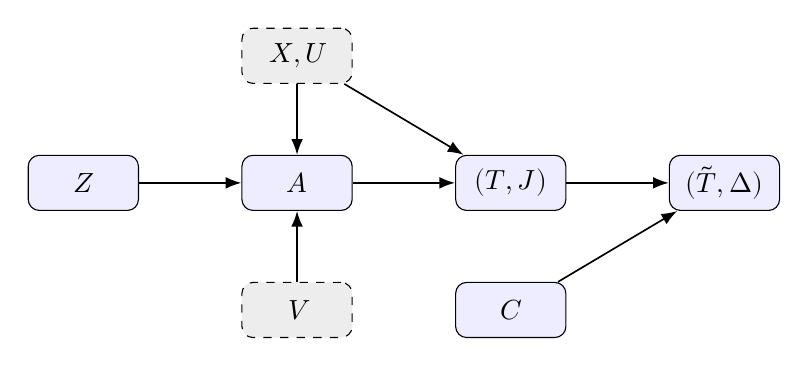
\begin{tikzpicture}[
  node distance=9mm and 13mm,
  observed/.style={draw,rounded corners,fill=blue!7,minimum width=14mm,minimum height=7mm,align=center},
  latent/.style={draw,dashed,rounded corners,fill=gray!14,minimum width=14mm,minimum height=7mm,align=center},
  arr/.style={-{Latex[length=2mm]},semithick}]
\node[observed] (z) {$Z$};
\node[observed,right=of z] (a) {$A$};
\node[observed,right=of a] (e) {$(T,J)$};
\node[observed,right=of e] (o) {$(\widetilde T,\Delta)$};
\node[latent,above=of a] (xu) {$X,U$};
\node[latent,below=of a] (v) {$V$};
\node[observed,below=of e] (c) {$C$};
\draw[arr] (z)--(a); \draw[arr] (a)--(e); \draw[arr] (e)--(o);
\draw[arr] (xu)--(a); \draw[arr] (xu)--(e); \draw[arr] (v)--(a);
\draw[arr] (c)--(o);
\end{tikzpicture}
\caption{Simulation data-generating structure. Dashed nodes are latent
to the unadjusted estimator. In the primary design, $C$ is generated
independently; the informative-censoring stress test adds dependence of
$C$ on $U$.}
\label{fig:dag}
\end{figure}

The horizon is $\tau=8$. Independent discrete censoring is calibrated
to 0\% or 30\% by period 10, and events win censoring ties. Because
$q_1-q_0=\delta(1-q_0)$, the complier distribution of $(X,U)$ does not
depend on $\delta$. Product Gauss--Hermite quadrature therefore gives
one deterministic truth for every positive instrument strength:
\[
\psi=\frac{E[(1-q_0)\{F_1^1(8\mid X,U)-F_1^0(8\mid X,U)\}]}
{E(1-q_0)}=-0.0964917269,
\qquad E(1-q_0)=0.7114055309.
\]
The value is stable beyond 12 decimal places from 40 through 80 nodes.

The fixed-strength experiment uses $n\in\{500,1000\}$,
$\delta\in\{0.05,0.15,0.35\}$, and 0\% or 30\% censoring. A direct
local-to-zero experiment uses
\[
n\in\{500,1000,2500,5000\},\qquad
\delta_n=\frac{c}{0.7114055309\sqrt n},\qquad
c\in\{0.5,1,2,4\},
\]
so that $\sqrt n\,\kappa_n=c$ exactly in expectation. Four additional
valid-design cells use 50\% or 65\% independent censoring. Eight paired
cells compare the exact finite-jump influence function with a
continuous-time/no-tie approximation. Finally, two informative-censoring
and two defier cells are labelled assumption-violation diagnostics and
are not evidence for the theorem. The 28 primary fixed-strength and
local-to-zero cells use 5,000 replications; the 16 supplementary cells
use 2,000, for 172,000 datasets in total. The master seed is 20260819.

Comparators use the same reduced-form and first-stage estimates: a
ratio-Wald interval divides by $\widehat\kappa$, whereas the score set
inverts the undivided moment. The code solves the quadratic inequality
exactly and records every connected component. Primary outcomes are
coverage, exact union length, full/disconnected/empty-set frequency,
and the median, 90th, 95th, and 99th percentiles of Wald length.

\section{Simulation results}

Table~\ref{tab:simulation} reports the fixed-strength results. A nominal
coverage estimate has Monte Carlo standard error about 0.003. Score
coverage is generally near 0.95 (0.9446--0.9534), with ordinary
finite-sample variation. Weak instruments make the set uninformative:
for $\delta=0.05$, its median length is the full feasible width 2 and
the full-set frequency is 0.721--0.806. Wald coverage is then close to
one only because its intervals have extreme tails, not because they are
informative. Means and ratio RMSE are omitted because rare
$\widehat\kappa\approx0$ replications make them non-reproducible
heavy-tail summaries.

\begin{table}[tbp]
\centering
\caption{Fixed-strength Monte Carlo results (5,000 replications per
cell). Length columns report medians except ``Wald p99.'' Score length
is the exact measure of the accepted union within $[-1,1]$.}
\label{tab:simulation}
\scriptsize
\setlength{\tabcolsep}{3.2pt}
\begin{tabular}{rrr r rrr rrr}
\toprule
$\delta$ & $n$ & Cens. & Mean $\widehat\kappa$ & \multicolumn{3}{c}{Score set} & \multicolumn{3}{c}{Ratio-Wald} \\
\cmidrule(lr){5-7}\cmidrule(lr){8-10}
&&&& Cov. & Length & Full & Cov. & Length & p99 \\
\midrule
0.05 & 500 & 0\% & 0.036 & 0.953 & 2.000 & 0.803 & 0.999 & 5.16 & 10582.5 \\
0.05 & 500 & 30\% & 0.036 & 0.948 & 2.000 & 0.806 & 0.999 & 5.48 & 4606.3 \\
0.05 & 1000 & 0\% & 0.035 & 0.949 & 2.000 & 0.721 & 0.999 & 3.76 & 2850.1 \\
0.05 & 1000 & 30\% & 0.036 & 0.946 & 2.000 & 0.734 & 0.999 & 3.92 & 4135.8 \\
0.15 & 500 & 0\% & 0.107 & 0.945 & 1.513 & 0.303 & 0.992 & 1.55 & 35.0 \\
0.15 & 500 & 30\% & 0.106 & 0.945 & 1.588 & 0.318 & 0.993 & 1.69 & 34.1 \\
0.15 & 1000 & 0\% & 0.107 & 0.947 & 1.159 & 0.071 & 0.978 & 1.08 & 3.8 \\
0.15 & 1000 & 30\% & 0.106 & 0.949 & 1.203 & 0.086 & 0.982 & 1.16 & 3.9 \\
0.35 & 500 & 0\% & 0.249 & 0.953 & 0.676 & 0.001 & 0.965 & 0.64 & 1.1 \\
0.35 & 500 & 30\% & 0.250 & 0.949 & 0.717 & 0.001 & 0.964 & 0.67 & 1.2 \\
0.35 & 1000 & 0\% & 0.249 & 0.945 & 0.461 & 0.000 & 0.951 & 0.45 & 0.6 \\
0.35 & 1000 & 30\% & 0.250 & 0.952 & 0.489 & 0.000 & 0.960 & 0.47 & 0.7 \\
\bottomrule
\end{tabular}
\end{table}

Figure~\ref{fig:local} is the direct check of the theorem's
local-to-zero regime. Across all 16 cells, score coverage is
0.9452--0.9554 and is approximately invariant in $n$ at fixed $c$.
Information, correctly, is governed by local strength: the full-set
frequency is 0.851--0.858 at $c=0.5$, 0.755--0.760 at $c=1$,
0.428--0.457 at $c=2$, and 0.021--0.027 at $c=4$.

\begin{figure}[tbp]
\centering

\includegraphics[width=.96\linewidth]{figures/local_coverage_informativeness.pdf}
\caption{Local-to-zero experiment under 30\% independent censoring.
Left: score-set coverage with pointwise 95\% Monte Carlo error bars.
Right: probability of the full feasible set. Each point uses 5,000
replications and $\sqrt n\,\kappa_n=c$ in expectation.}
\label{fig:local}
\end{figure}

Figure~\ref{fig:tails} shows why a mean Wald length is a poor diagnostic.
At $n=1000$ and 30\% censoring, the 99th percentile is 4136 for
$\delta=0.05$ but only 0.69 for $\delta=0.35$; the score set is bounded
by the feasible width 2. Figure~\ref{fig:topology} additionally shows
that disconnected sets occur in up to 1.94\% of weak-IV replications
and empty feasible sets in up to 0.08\%. Replacing the set by its convex
hull would therefore change actual simulation output.

\begin{figure}[tbp]
\centering
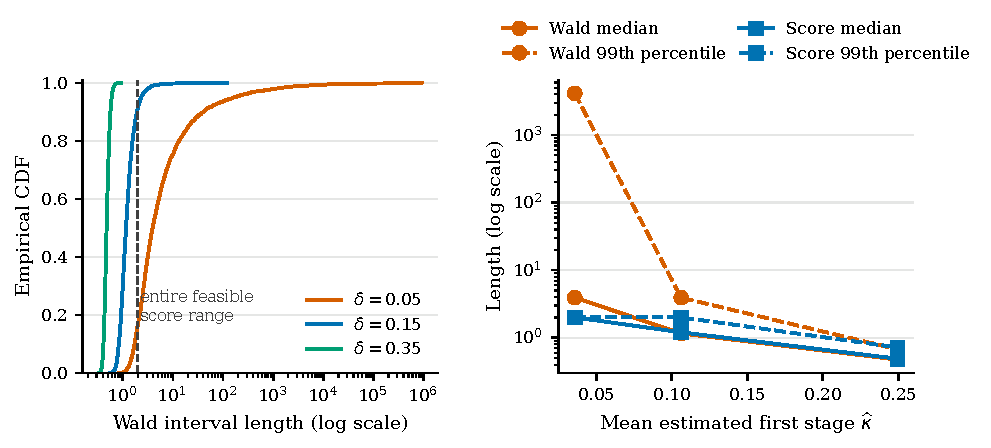
\includegraphics[width=.98\linewidth]{figures/denominator_instability.pdf}
\caption{Near-zero-denominator pathology in the fixed-strength design
($n=1000$, 30\% censoring). Left: empirical distributions of Wald
length. Right: median and 99th-percentile lengths for Wald intervals and
score sets. Both axes reporting length use logarithmic scaling where
indicated.}
\label{fig:tails}
\end{figure}

\begin{figure}[tbp]
\centering

\includegraphics[width=.96\linewidth]{figures/score_set_topology.pdf}
\caption{Exact topology of the score-inverted confidence set in the
fixed-strength experiment. ``Ordinary interval'' excludes the full set;
the small disconnected and empty categories are retained rather than
collapsed to a convex hull.}
\label{fig:topology}
\end{figure}

The additional valid-design experiments tell the same story. At 50\%
and 65\% independent censoring, score coverage is 0.9405--0.9455; median
length increases to 1.261--1.684. In the four paired tie ablations, the
finite-jump correction changes estimated score coverage by only
0.0010--0.0025 at the hazards used, but it is retained because it is the
correct influence representation for the discrete design. The
informative-censoring and defier experiments are diagnostics only: their
numerical coverage does not restore the causal interpretation lost when
A6 or monotonicity fails.

\section{Practical implications and limitations}

Analysts should report the estimated compliance contrast, the score
confidence set, whether the set is disconnected or full, and the
competing-risk and censoring conventions. A narrow ratio-Wald interval
should not be reported merely after screening on a first-stage
threshold; such pretesting changes the inferential procedure. The method
is appropriate for randomized encouragement studies or similarly
defensible binary IVs with independent censoring within instrument arm.

The method should not be used without modification when censoring
depends on treatment or covariates, instruments or providers create
clustering, treatment is time varying, monotonicity is implausible,
exclusion is violated, or the target is a direct effect unaffected by
competing events. Covariate-adjusted and cross-fitted extensions are
plausible but not proved here. Exact-zero compliance leaves the complier
effect undefined; the theorem concerns sequences with positive $\kappa_n$.

\section{Conclusion}

For a fixed-horizon cause-specific complier cumulative-incidence effect,
the inferentially consequential step is not another ratio estimator but
avoidance of ratio linearization. Inverting the joint
Aalen-Johansen/treatment-uptake score gives valid uncertainty under
local-to-zero compliance, provided the usual competing-risk and IV
assumptions hold. The price of honesty is an uninformative set when the
design contains little causal information.

\section*{References}

Aalen, O. O., and Johansen, S. (1978). An empirical transition matrix
for non-homogeneous Markov chains based on censored observations.
\emph{Scandinavian Journal of Statistics}, 5, 141-150.

Ailer, E., Hartford, J., and Kilbertus, N. (2023). Sequential
underspecified instrument selection for cause-effect estimation.
\emph{Proceedings of the 40th International Conference on Machine
Learning}, PMLR 202. https://proceedings.mlr.press/v202/ailer23a.html

Allignol, A., Schumacher, M., and Beyersmann, J. (2010). A note on
variance estimation of the Aalen-Johansen estimator of the cumulative
incidence function in competing risks, with a view towards
left-truncated data. \emph{Biometrical Journal}, 52, 126-137.
https://doi.org/10.1002/bimj.200900039

Anderson, T. W., and Rubin, H. (1949). Estimation of the parameters of a
single equation in a complete system of stochastic equations.
\emph{Annals of Mathematical Statistics}, 20, 46-63.
https://doi.org/10.1214/aoms/1177730090

Beyersmann, J., Di Termini, S., and Pauly, M. (2013). Weak convergence
of the wild bootstrap for the Aalen-Johansen estimator of the cumulative
incidence function of a competing risk. \emph{Scandinavian Journal of
Statistics}, 40, 387-402.
https://doi.org/10.1111/j.1467-9469.2012.00817.x

Beyhum, J., Florens, J.-P., and Van Keilegom, I. (2023). A nonparametric
instrumental approach to confounding in competing risks models.
\emph{Lifetime Data Analysis}, 29, 611-641.
https://doi.org/10.1007/s10985-023-09599-3

Fieller, E. C. (1954). Some problems in interval estimation.
\emph{Journal of the Royal Statistical Society: Series B
(Methodological)}, 16(2), 175--185.
https://doi.org/10.1111/j.2517-6161.1954.tb00159.x

Hartford, J., Veitch, V., Sridhar, D., and Leyton-Brown, K. (2021).
Valid causal inference with (some) invalid instruments.
\emph{Proceedings of the 38th International Conference on Machine
Learning}, PMLR 139. https://proceedings.mlr.press/v139/hartford21a.html

Kjaersgaard, M. I. S., and Parner, E. T. (2016). Instrumental variable
method for time-to-event data using a pseudo-observation approach.
\emph{Biometrics}, 72, 463-472. https://doi.org/10.1111/biom.12451

Kuang, Z., Sala, F., Sohoni, N., Wu, S., Cordova-Palomera, A., Dunnmon,
J., Priest, J., and Re, C. (2020). Ivy: Instrumental variable synthesis
for causal inference. \emph{Proceedings of the 23rd International
Conference on Artificial Intelligence and Statistics}, PMLR 108.
https://proceedings.mlr.press/v108/kuang20a.html

Lee, Y., Kennedy, E. H., and Mitra, N. (2023). Doubly robust
nonparametric instrumental variable estimators for survival outcomes.
\emph{Biostatistics}, 24, 518-537.
https://doi.org/10.1093/biostatistics/kxab036

Liu, T., Lawlor, P., Ungar, L., and Kording, K. (2022). Data-driven
exclusion criteria for instrumental variable studies. \emph{Proceedings
of the First Conference on Causal Learning and Reasoning}, PMLR 177.
https://proceedings.mlr.press/v177/liu22a.html

Ma, Y. (2026). Identification-robust inference for the LATE with
high-dimensional covariates. \emph{Journal of Econometrics}, 257,
106302. https://doi.org/10.1016/j.jeconom.2026.106302; arXiv:2302.09756.

Richardson, A., Hudgens, M. G., Fine, J. P., and Brookhart, M. A.
(2017). Nonparametric binary instrumental variable analysis of competing
risks data. \emph{Biostatistics}, 18, 48-61.
https://doi.org/10.1093/biostatistics/kxw023

Smucler, E., Lanni, J., and Masip, D. (2025). A note on the properties
of the confidence set for the local average treatment effect obtained by
inverting the score test. arXiv:2506.10449.
https://arxiv.org/abs/2506.10449

Zheng, C., Dai, R., Hari, P. N., and Zhang, M.-J. (2017). Instrumental
variable with competing risk model. \emph{Statistics in Medicine},
36(8), 1240--1255. https://doi.org/10.1002/sim.7205

\appendix
\section{Proof of the finite-grid theorem}

Let $W(O)$ collect the finitely many bounded indicators
\[
I(Z=z),\quad I(Z=z)A,\quad
I(Z=z)Y(k),\quad I(Z=z)N_\ell(k),
\]
for $z\in\{0,1\}$, $k=1,\ldots,L$, and
$\ell=1,\ldots,K$. All empirical arm probabilities, risk probabilities,
hazards, treatment proportions, and Aalen--Johansen cumulative
incidences are functions of
\[
q_P=E_P\{W(O)\},\qquad \widehat q=\mathbb P_nW.
\]
On the set defined by A2 and A7, these functions are twice continuously
differentiable, and their first and second derivatives are uniformly
bounded. A uniform second-order Taylor expansion therefore gives
\[
\sqrt n(\widehat\theta-\theta_P)
=\frac{1}{\sqrt n}\sum_{i=1}^n\Phi_{\theta,P}(O_i)+R_{n,P},
\qquad
\sup_{P\in\mathcal P}\Pr_P(\|R_{n,P}\|>\eta)\longrightarrow0
\]
for every $\eta>0$, where
$\theta_P=(F_{1j},F_{0j},p_1,p_0)^\mathsf T$. Indeed, because $W$ has
fixed dimension and bounded coordinates,
$\|\widehat q-q_P\|=O_P(n^{-1/2})$ uniformly, while the Taylor remainder
is $O_P\{\sqrt n\|\widehat q-q_P\|^2\}=O_P(n^{-1/2})$.

The influence function of the arm-specific hazard is
\[
\frac{I(Z=z)}{\pi_zH_z(k)}
\{N_\ell(k)-Y(k)\alpha_{z\ell}(k)\}.
\]
Differentiating
$F_{zj}(\tau)=\sum_{k=1}^L S_z(t_k-)\alpha_{zj}(k)$ gives
\[
dF_{zj}(\tau)
=\sum_{k=1}^L S_z(t_k-)\,d\alpha_{zj}(k)
-\sum_{k=1}^L
\frac{F_{zj}(\tau)-F_{zj}(t_k)}
{1-\alpha_{z\cdot}(k)}\,d\alpha_{z\cdot}(k).
\]
Substitution yields \eqref{eq:discrete-aj-if}. The
treatment-proportion derivative is $I(Z=z)(A-p_z)/\pi_z$. Since $h_b$
is linear in $\theta_P$, its influence function is
$g_{b,P}=\Phi_{N,P}-b\Phi_{\kappa,P}$, proving the stated uniform
asymptotic-linear expansion.

The plug-in influence functions are continuous functions of
$\widehat q$. Uniform consistency of $\widehat q$, boundedness, and the
finite-dimensional law of large numbers imply
\[
\sup_{b\in[-1,1]}
\left|\mathbb P_n\widehat g_b^2-E_Pg_{b,P}^2\right|=o_P(1)
\]
uniformly over $\mathcal P$. At $b=\psi(P)$, identification implies
$h_b(P)=N_j-\psi(P)\kappa=0$. The influence functions are uniformly
bounded under A2 and A7, and their variances at the truth are bounded
below under A8. Hence the Berry--Esseen bound applies uniformly:
\[
\sup_{P\in\mathcal P}\sup_x
\left|
\Pr_P\!\left[
\frac{\sum_{i=1}^n g_{\psi(P),P}(O_i)}
{\sqrt{nE_Pg_{\psi(P),P}^2}}\le x
\right]-\Phi(x)
\right|\longrightarrow0.
\]
Combining this result with asymptotic linearity and variance consistency
yields $T_n\{\psi(P)\}\Rightarrow\chi^2_1$ uniformly over
$\mathcal P$. Inverting the test proves coverage. No step divides by
$\kappa(P)$.

\section{Reproducibility}

Run
\begin{verbatim}
python simulate_weak_iv_cif_extended.py --output extended_results_final \
  --replications 2000 --primary-replications 5000 --workers 4
python make_simulation_figures.py
\end{verbatim}
The simulation writes aggregate results, replicate-level diagnostics,
and JSON metadata including software versions, arguments, seed,
quadrature stability, and wall-clock runtime. Replicate output contains
both score components, quadratic coefficients, variance terms,
$\widehat N$, $\widehat\kappa$, and Wald endpoints. The figure script
reconstructs every plotted quantity from those files. No training or
tuning data are used because no machine-learning nuisance estimator is
fitted.

\end{document}
